\subsection{Versionsstyring}
Under udviklingen af spillet er der blevet anvendt versionsstyring i form a git og et "repository" på Github. Repository'et kan findes her: \url{https://github.com/ExoHumann/40_del3}
På github kan den seneste version af spillet findes. 

\vspace{.5cm}
Der er derudover også blevet anvendt versionsstyring til dokumentationen(dette dokument) her er der også blevet anvendt git og Github. Repository'et kan findes her:
\url{https://github.com/joha413/CDIO3-rapport}
Det er her at den seneste version af dokumentationen kan findes.

\subsection{Hent og byg spillet}
Når man gerne vil hente og bygge spillet med Intellij IDEA(\cite{noauthor_intellij_nodate}) Åbner man Intellij og trykker: File \textrightarrow New \textrightarrow Project from Version Control. Derefter kopiere man git repository url ind fra github (figur \ref{fig:github}). Derefter trykker man Clone
\begin{figure}[H]
    \centering
    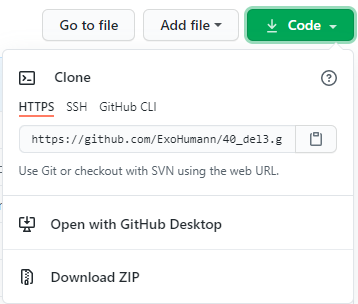
\includegraphics{sources/github.PNG}
    \caption{Github repository klon værktøjer}
    \label{fig:github}
\end{figure}

Når projektet er åbnet i Intellij trykker man på den grønne hammer(eller ctrl+f9) for at bygge projektet.
